\documentclass[rep.tex]{subfiles}
\begin{document}

\chapter{Zadanie 1}
\section{Treść}
Udowodnić, że powietrzna linia współosiowa o stosunku promieni
przewodów zewnętrznego do wewnętrznego równym
$\sqrt{e} = 1.648721271\ldots$ może przenosić falę
elektromagnetyczną o największej mocy.
Zadaną wielkością jest maksymalne natężenie pola elektrycznego,
przy którym następuje przebicie elektryczne wypełniającego
linię powietrza.

\section{Rozwiązanie}
\begin{figure}[!htbp]
  \centering
  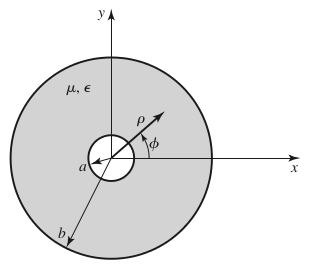
\includegraphics[scale=0.5]{fig/zad1/coax}
  \caption{Przekrój przez linie współosiową oraz symbole jej parametrów}
  \label{fig:zad1:coax}
\end{figure}

Współosiową linie transmisyjną pokazano na rysunku~\ref{fig:zad1:coax}.
W treści zadania powiedziano, że mamy doczynienia z linią powietrzną więc $\epsilon = \epsilon_0$ oraz $\mu = \mu_0$.
Moc fali przenoszonej przez linie jest równa:
\begin{equation}
  P = \oint_S\bar{E}(x, y) \times \bar{H}(x, y) \; \mathrm{ds}
\end{equation}
Ponieważ wyrażenia na pole elektryczne i magnetyczne w kartezjańskim układzie współrzędnych byłyby bardzo skomplikowane,
należy zmienić układ współrzędnych na polarny:
\begin{equation}
  P = \frac{1}{2} \int\limits_0^{2\pi}\int\limits_a^b \bar{E}(\rho, \phi) \cdot \bar{H}(\rho, \phi) \rho \; \mathrm{d\rho} \mathrm{d\phi}
\end{equation}
Pole elektryczne i magnetyczne mają postać:
\begin{align}
  \bar{E}(\rho)    & = \frac{U_0\hat{\rho}}{\rho \ln \frac{b}{a}} \\
  \bar{H}(\phi) & = \frac{\bar{E}(\rho)\hat{\phi}}{\eta_0}
\end{align}
gdzie: \\
\begin{tabular}{l @{ - } l}
  $\hat{\rho}$ & wersor w kierunku $\rho$, \\
  $\hat{\phi}$ & wersor w kierunku $\phi$, \\
  $\xi_0 = \sqrt{\frac{\mu_0}{\epsilon_0}}$ & impedancja falowa linii. \\
\end{tabular}

Możemy teraz policzyć moc fali przenoszonej przez linie:
\begin{align}
  P & =  \frac{1}{2} \int\limits_0^{2\pi}\int\limits_a^b \bar{E}(\rho, \phi) \cdot \bar{H}(\rho, \phi) \rho \; \mathrm{d\rho} \mathrm{d\phi} \nonumber \\
    & =  \frac{1}{2} \int\limits_0^{2\pi}\int\limits_a^b \frac{1}{\xi_0}\frac{U_0^2}{\rho^2\ln^2\frac{b}{a}} \rho \; \mathrm{d\rho} \mathrm{d\phi} \nonumber \\
    & =  \frac{1}{2} \int\limits_0^{2\pi}\int\limits_a^b \frac{1}{\xi_0}\frac{U_0^2}{\rho\ln^2\frac{b}{a}} \; \mathrm{d\rho} \mathrm{d\phi} \nonumber \\
    & =  \frac{1}{2} \frac{1}{\xi_0}\frac{U_0^2}{\ln^2\frac{b}{a}} \int\limits_0^{2\pi}\int\limits_a^b \frac{1}{\rho} \; \mathrm{d\rho} \mathrm{d\phi} \nonumber \\
    & =  \frac{1}{2} \frac{1}{\xi_0}\frac{U_0^2}{\ln^2\frac{b}{a}} \int\limits_0^{2\pi} \ln|\rho|\Big\arrowvert_a^b \; \mathrm{d\phi} \nonumber \\
    & =  \frac{1}{2} \frac{1}{\xi_0}\frac{U_0^2}{\ln^2\frac{b}{a}} \ln\frac{b}{a} \int\limits_0^{2\pi} 1 \; \mathrm{d\phi} \nonumber \\
    & =  \frac{1}{2} \frac{1}{\xi_0}\frac{U_0^2}{\ln\frac{b}{a}} \phi\Big\arrowvert_0^{2\pi} \nonumber \\
    & =  \frac{2\pi}{\xi_0}\frac{U_0^2}{\ln\frac{b}{a}} \label{eqn:zad1:power}
\end{align}

Korzystając z zależności:
\begin{equation}
  U_0 = E_{max}\cdot a \ln\frac{b}{a} \label{eqn:zad1:emax}
\end{equation}
można wyznaczyć moc fali propagującej się w lini w zależności od maksymalnego natężenia pola elektromagnetycznego ($E_{max}$).
Podstawuając~\ref{eqn:zad1:emax} do~\ref{eqn:zad1:power} otrzymuję się:
\begin{align}
  P &= \frac{2\pi}{\xi_0}\frac{E_{max}^2 \cdot a^2 \ln^2\frac{b}{a}}{\ln\frac{b}{a}} \nonumber \\
    &= \frac{2\pi}{\sqrt{\frac{\mu_0}{\epsilon_0}}}E_{max}^2 \cdot a^2 \ln\frac{b}{a} \nonumber \\
    &= \underbrace{2\pi\sqrt{\frac{\epsilon_0}{\mu_0}}E_{max}^2}_K \; \cdot a^2 \ln\frac{b}{a} \nonumber \\
    &= K \cdot a^2 \ln\frac{b}{a} \label{eqn:zad1:pow}
\end{align}
$K$ we wzorze~\ref{eqn:zad1:pow} jest stałe, zależne tylko od podanego w zadaniu maksymalnego natężenia pola.

Moc fali propagującej się w linii będzie maksymalna gdy pochodna mocy określonej wzorem~\ref{eqn:zad1:pow}~($\frac{\mathrm{dP(a)}}{\mathrm{da}}$)
będzie równa $0$.
\begin{align}
  \frac{\mathrm{dP(a)}}{\mathrm{da}} &= K \cdot 2a\ln\frac{b}{a} + K \cdot a^2(-\frac{1}{a}) \nonumber \\
    &= Ka[2\ln\frac{b}{a} - 1] \label{eqn:zad1:dp}
\end{align}
Wyrażenie~\ref{eqn:zad1:dp} jest równe $0$ gdy $2\ln\frac{b}{a} - 1 = 0$.
Co z kolei przekłada się na warunek $\ln\frac{b}{a} = \frac{1}{2}$, który jest spełniony gdy $\frac{b}{a} = \sqrt{\mathrm{e}}$,
co należało dowieść.

\end{document}
